\documentclass[12pt]{article}
\usepackage{amsmath}
\usepackage{amssymb}
\usepackage{amsthm}
\usepackage{accents}
\usepackage{graphicx}
\usepackage{amsfonts}
\setlength{\oddsidemargin}{0in}
\setlength{\textwidth}{6.5in}
\setlength{\topmargin}{-.55in}
\setlength{\textheight}{9in}
\pagestyle{empty}
\renewcommand \d{\displaystyle}
\begin{document}
\noindent Dallas Klumpe

\noindent Math 4310

\noindent HW 4\\

Section 28\\

1. For each of the following functions defined on $\mathbb{R}$, give the set of points at which it is not differentiable.\\
c. $|\sin x|$. This function is not differentiable at every point where $\sin x=0$. So, $|\sin x|$ is not differentiable at the points$\{x|x=n\pi,n\in\mathbb{Z}\}$.\\
f. $|x^3-8|$. This function is not differentiable at every point where $x^3-8=0$. So, $|x^3-8|$ is not differentiable at the point $x=2$.\\[20pt]

4. Let $f(x)=x^2\sin{\frac{1}{x}}$ for $x\neq0$ and $f(0)=0$.\\
a. Use Theorems 28.3 and 28.4 to show $f$ is differentiable at every $a\neq0$ and calculate $f'(a)$.\\
Let $a\in\mathbb{R}\setminus\{0\}$. Now, clearly $x^2$, $\sin x$, and $\frac1x$ are differentiable at all $x=a$. So, by Theorem 28.4, we have that $\sin{\frac1x}$ is differentaible at all $x=a$ and then by Theorem 28.3, we have that $x^2\sin{\frac1x}$ is differentiable at all $a\neq0$. So, $f'(a)$ exists, and $f'(a)=2x\sin{\frac1x}+x^2\cos{\frac1x}(-\frac{1}{x^2})=2x\sin{\frac1x}-\cos({\frac1x})$.\\
b. Use the definition to show that $f$ is differentiable at $x=0$ and $f'(0)=0$.\\
Take $\frac{f(x)-f(0)}{x-0}$. Well, this becomes $\frac{x^2\sin{\frac{1}{x}}-0}{x-0}=\frac{x^2\sin{\frac{1}{x}}}{x}=x\sin{\frac{1}{x}}$. Now, $\lim_{x\rightarrow0}x\sin{\frac{1}{x}}=0$ since $-1\leq sin(\frac1x)\leq1$. Since the limit exists and is finite, $f'(0)$ exists and in particular $f'(0)=0$.\\
c. Show $f'$ is not continuous at $x=0$.\\
Take the sequence $s_n=\frac{1}{n}$. Clearly $\lim_{n\rightarrow\infty}s_n=0$, however we have that $\lim_{n\rightarrow\infty}f'(s_n)=\lim_{n\rightarrow\infty}s_n\sin(\frac{1}{s_n})=\lim_{n\rightarrow\infty}\frac{\sin n}{n}=1\neq0$. Thus, $f'(x)$ not continuous at $x=0$.\\[20pt]

5. Let $f(x)=x^2\sin{\frac{1}{x}}$ for $x\neq0$, $f(0)=0$, and $g(x)=x$ for $x\in\mathbb{R}$.\\
a. Observe $f$ and $g$ are differentiable on $\mathbb{R}$.\\
Clearly $g$ is differentiable on $\mathbb{R}$, and by above , we know that $f$ is also differentiable on $\mathbb{R}$.\\
b. Calculate $f(x)$ for $x=\frac{1}{n\pi}$, $n\in\mathbb{Z^+}\cup\mathbb{Z^-}$.\\
Well, for $x=\frac{1}{n\pi}$, $n\in\mathbb{Z^+}\cup\mathbb{Z^-}$, $f(x)=(\frac{1}{n\pi})^2\sin{n\pi}=0$ as we reccognized above that $\sin n\pi=0$ for $n\in\mathbb{Z}$.\\
c. Explain why $\lim_{x\rightarrow0}\frac{g(f(x))-g(f(0))}{f(x)-f(0)}$ is meaningless.\\
Well, $g(x)=x$ is the identity with respect to composition, so the above limit becomes $\lim_{x\rightarrow0}\frac{f(x)-f(0)}{f(x)-f(0)}=\lim_{x\rightarrow0}1=1$ which tells us nothing about the functions.\\[20pt]

7. Let $f(x)=x^2$ for $x\geq0$ and $f(x)=0$ for $x<0$.\\
a. \begin{center}
	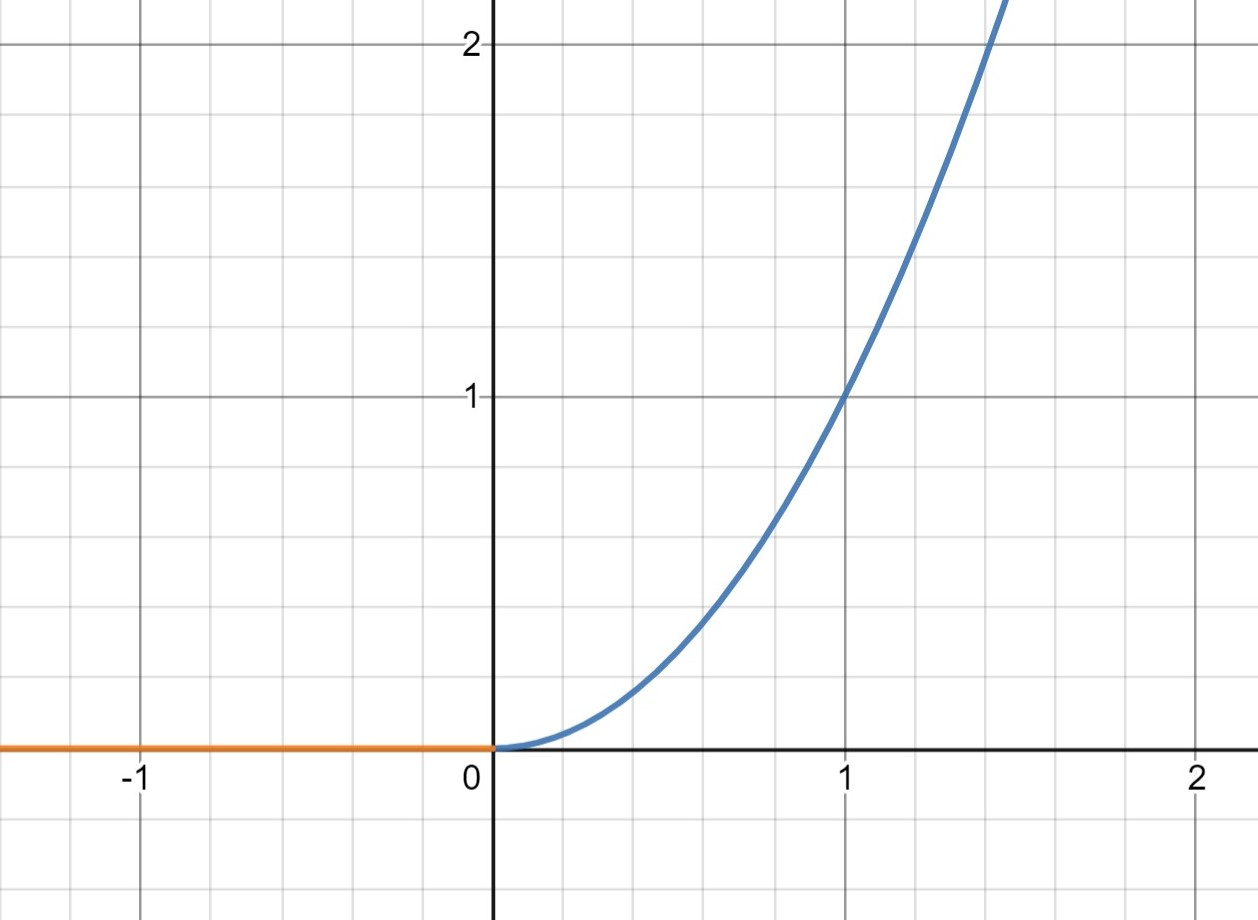
\includegraphics[scale=1]{graph.JPG}\\
\end{center}
\vspace{\stretch{1}}
b. Show $f$ is differentiable at $x=0$.\\
Well, take $\frac{f(x)-f(0)}{x-0}$. Then $\lim_{x\rightarrow0^-}\frac{f(x)-f(0)}{x-0}=\lim_{x\rightarrow0^-}\frac{0-0}{x-0}=0$. Also, $\lim_{x\rightarrow0^+}\frac{f(x)-0}{x-0}=\lim_{x\rightarrow0^+}\frac{x^2}{x}=\lim_{x\rightarrow0^+}x=0$. Since the limit exists, is the same from both directions, and is finite, we get that $f$ is differentiable at $x=0$. In particular $f'(0)=0$\\
c. Calculate $f'$ on $\mathbb{R}$.\\
Well $\frac{d}{dx}x^2=2x$ and $\frac{d}{dx}0=0$, so $f'(x)=2x$ for $x\geq0$ and $f'(x)=0$ for $x<0$.\\
d. Is $f'$ continuous on $\mathbb{R}$? DIfferentiable on $\mathbb{R}$?\\
Well take any sequence $s_n$ such that $\lim_{n\rightarrow\infty}s_n=0$ where $s_n\neq0$ for all $n$. Then $\lim_{n\rightarrow\infty}f(s_n)=\lim_{n\rightarrow\infty}2s_n=2\lim_{n\rightarrow\infty}s_n=2*0=0=f(0)$. Thus, $f'$ is continuous at $x=0$ and by continuity of ploynomials, is continuous everywhere else. $f$ is not differentiable on $\mathbb{R}$ as $\lim_{x\rightarrow0^-}\frac{f(x)-f(0)}{x-0}=0\neq1=\lim_{x\rightarrow0^+}\frac{f(x)-f(0)}{x-0}$.\\[20pt]

Section 29\\

4. Let $f$ and $g$ be differentiable functions on an open interval $I$. Suppose $a,b\in I$ satisfy $a<b$ and $f(a)=f(b)=0$. Show $f'(x)+f(x)g'(x)=0$ for some $x\in(a, b)$.\\
Let $f$, $g$, $a$, and $b$ be as given. Consider $h(x)=f(x)e^{g(x)}$. Well $h(a)=h(b)=0$ by assumption. So, by Rolle's Theorem, we have that $f'(x)e^{g(x)}+f(x)e^{g(x)}g'(x)=0$ for some $x\in I$. Dividing by $e^{g(x)}$, we get $f'(x)+f(x)g'(x)=0$ for some $x\in(a, b)$ since $e^{g(x)}\neq0$.\\[20pt]

5. Let $f$ be defined on $\mathbb{R}$, and suppose $|f(x)-f(y)|\leq(x-y)^2$ for all $x,y\in\mathbb{R}$. Prove $f$ is a constant function.\\
Let $f$ be as given above and let $x,y\in\mathbb{R}$. Then we can rewrite this as $|f(x)-f(y)|\leq|x-y||x-y|$. Hence, $|\frac{f(x)-f(y)}{x-y}|\leq|x-y|$. Well, $|f'(y)|=\lim_{x\rightarrow y}|\frac{f(x)-f(y)}{x-y}|\leq\lim_{x\rightarrow y}|x-y|=|y-y|=0$. Thus, $f'(y)=0$ and since $y$ was arbitrary, we have that $f'(x)=0$ for all $x\in\mathbb{R}$. So, by corollary 29.4 we have that $f(x)$ is a constant function on $\mathbb{R}$.\\[20pt]

7.a. Suppose $f$is twice differentiable on an open interval $I$ and $f''(x)=0$ for all $x\in I$. Show $f$ has the form $f(x)=ax+b$ for suitable constants $a$ and $b$.\\
Let $f$ and $I$ be as given. Since $f''(x)=0$ for all $x\in I$, we know that $f'(x)=a$ for all $x\in I$ for some constant $a$ by corollary 29.4. Now, let $g(x)=ax$. We then see that $f'(x)=g'(x)$ for all $x\in I$. So, by corollary 29.5, we have that $f(x)=g(x)+b=ax+b$ for some constant $a$ and a suitable constant $b$.\\
b.Suppose $f$ is three times differentiable on an open interval $I$ and $f'''(x)=0$ on $I$. What form does $f$ have? Prove your claim.\\
Well, we know that $f'(x)=ax+b$ for suitable constants $a$ and $b$. Now, let $h(x)=\frac{a}{2}x^2+bx$. We then see that $h'(x)=ax+b=f'(x)$. So, by corollary 29.5, we see that $f(x)=h(x)+c=\frac{a}{2}x^2+bx+c$ for appropriate constants $a ,b$, and $c$.\\[20pt]

11. Show $\sin x\leq x$ for all $x\geq0$.\\
Let $f(x)=x-\sin x$. Well, $f'(x)=1-\cos x$. Now since $|\cos x|\leq1$, we have that $f'(x)\geq0$ for all $x\geq0$. % where equality holds for $x=2n\pi$ for $$.% 
So, $f(x)$ is an increasing function on $[0,\infty)$. That means $x-\sin x\geq0$ so $\sin x\leq x$ for all $x\geq0$\\[20pt]

15. Let $r$ be a nonzero rational number $\frac{m}{n}$ where $n$ is a positive integer, $m$ is any nonzero integer, and $m$ and $n$ have no common factors. Let $h(x)=x^r$ where $dom(h)=[0,\infty)$ if $n$ is even and $m>0$, $dom(h)=(0,\infty)$ if $n$ is even and $m<0$, $dom(h)=\mathbb{R}$ if $n$ is odd and $m>0$, and $dom(h)=\mathbb{R}\setminus{0}$ if $n$ is odd and $m<0$. Show $h'(x) = rx^{r-1}$ for $x\in dom(h), x\neq0$.\\
Let $r$ be as given and $x\in dom(h)$ with $x\neq0$. Then $h(x)=x^r=x^{\frac{m}{n}}=(x^{\frac1n})^m$. So, $h'(x)=m(x^{\frac1n})^{m-1}(\frac1nx^{\frac1n-1})$ by the chain rule and example 2 in the book. Hence, $m(x^{\frac1n})^{m-1}(\frac1nx^{\frac1n-1})=\frac{m}{n}x^{\frac{m-1}{n}}x^{\frac1n-1}=\frac{m}{n}x^{\frac{m-1}{n}+\frac1n-1}=\frac{m}{n}x^{\frac{m}{n}-1}=rx^{r-1}$ as desired.\\[20pt]

18. Let $f$ be differentiable on $\mathbb{R}$ with $a=sup\{|f'(x)|:x\in\mathbb{R}\}<1$.\\
a. Select $s_0\in\mathbb{R}$ and define $s_n=f(s_{n-1})$ for $n\geq1$. Thus $s_1=f(s_0)$, $s_2=f(s_1)$, etc. Prove $s_n$ is a convergent sequence.\\
Well, since $f$ is differentiable on $\mathbb{R}$, we have that $f$ is continuous on $\mathbb{R}$ as well. Therefore on the interval $(s_n, s_{n-1})$ there exists $x\in(s_n, s_{n-1})$ such that $f'(x)=\frac{f(s_n)-f(s_{n-1})}{s_n-s_{n-1}}$. By assumption, we then have $|\frac{f(s_n)-f(s_{n-1})}{s_n-s_{n-1}}|=|\frac{s_{n+1}-s_n}{s_n-s_{n-1}}|=|f'(x)|\leq a$. Hence $|s_{n+1}-s_n|\leq a|s_n-s_{n+1}|$. So, $|s_n-s_m|=|s_n-s_{n-1}+s_{n-1}-s_{n-2}+...+s_{m+1}-s_m|\leq|s_n-s_{n-1}|+|s_{n-1}-s_{n-2}|+...+|s_{m+1}-s_m|\leq a^{n-1}|s_1-s_0|+a^{n-2}|s_1-s_0|+...+a^m|s_1-s_0|=(a^{n-1}+a^{n-2}+...+a^m)|s_1-s_0|\leq\frac{a^m}{1-a}|s_1-s_0|$. Let $\epsilon>0$ and let $N\in\mathbb{N}$ with $m,n>N$. Since $a<1$, we have $a^m<a^N$. Let $\epsilon=\frac{a^N}{1-a}|s_1-s_0|$. Since $s_1\neq s_0$, we have $|s_n-s_m|\leq\frac{a^m}{1-a}|s_1-s_0|<\frac{a^N}{1-a}|s_1-s_0|=\epsilon$. So, the sequence $(s_n)$ is Cauchy and therefore convergent.\\
b. Show $f$ has a fixed point.\\
Since we know that the sequence $s_n$ converges, lets set $\lim_{n\rightarrow\infty}s_n=c$ where $c\in\mathbb{R}$. Now, $f(s_n)=s_{n+1}$, so $\lim_{n\rightarrow\infty}f(s_n)=\lim_{n\rightarrow\infty}s_{n+1}=\lim_{n\rightarrow\infty}s_n=c$. Thus we have that $f(c)=c$, and so $f$ has a fixed point as desired.\\[20pt]

Section 30\\

2.c. Find the limit of $\lim_{x\rightarrow0}(\frac{1}{\sin x}-\frac{1}{x})$ if it exists.\\
$\lim_{x\rightarrow0}(\frac{1}{\sin x}-\frac{1}{x})=\lim_{x\rightarrow0}\frac{x-\sin x}{x\sin x}=\frac00$. By L'Hospitals rule, we get $\lim_{x\rightarrow0}\frac{x-\sin x}{x\sin x}=\lim_{x\rightarrow0}\frac{1-\cos x}{\sin x+x\cos x}=\frac{1-1}{0+0}=\frac00$. By L'Hospitals rule again, we get $\lim_{x\rightarrow0}\frac{x-\sin x}{x\sin x}=\lim_{x\rightarrow0}\frac{1-\cos x}{\sin x+x\cos x}=\lim_{x\rightarrow0}\frac{\sin x}{\cos x-x\sin x+\cos x}=\frac02=0$. So, $\lim_{x\rightarrow0}(\frac{1}{\sin x}-\frac{1}{x})=0$.\\[20pt]

3. Find the following limits if they exist.\\
a. $\lim_{x\rightarrow\infty}\frac{x-\sin x}{x}$\\
$\lim_{x\rightarrow\infty}\frac{x-\sin x}{x}=\lim_{x\rightarrow\infty}1-\frac{\sin x}{x}=1-\lim_{x\rightarrow\infty}\frac{\sin x}{x}$. Since $\lim_{x\rightarrow\infty}\frac{\sin x}{x}=0$ becasue $|\sin x|\leq1$, we have $1-\lim_{x\rightarrow\infty}\frac{\sin x}{x}=1-0=1$.\\
b. $\lim_{x\rightarrow0}\frac{1-\cos2x-2x^2}{x^4}$.\\
$\lim_{x\rightarrow0}\frac{1-\cos2x-2x^2}{x^4}=0$, so $\lim_{x\rightarrow0}\frac{1-\cos2x-2x^2}{x^4}=\lim_{x\rightarrow0}\frac{2\sin2x-4x}{4x^3}=\lim_{x\rightarrow0}\frac{4\cos2x-4}{12x^2}=\lim_{x\rightarrow0}\frac{-8\sin2x}{24x}=\lim_{x\rightarrow0}\frac{-16\cos2x}{24}=-\frac{16}{24}=-\frac23$\\[20pt]

5. Find the limit of $\lim_{x\rightarrow\infty}(e^x+x)^{\frac1x}$.\\
Well, $\lim_{x\rightarrow\infty}(e^x+x)^{\frac1x}=e^{\lim_{x\rightarrow\infty}\ln((e^x+x)^{\frac1x})}=e^{\lim_{x\rightarrow\infty}\frac1x\ln(e^x+x)}=e^{\lim_{x\rightarrow\infty}\frac{\ln(e^x+x)}{x}}=e^{\lim_{x\rightarrow\infty}\frac{e^x+1}{e^x+x}}=e^{\lim_{x\rightarrow\infty}\frac{e^x}{e^x+1}}=e^{\lim_{x\rightarrow\infty}\frac{e^x}{e^x}}=e^1=e$.





\end{document}